\documentclass{article} 
\usepackage{graphicx}
\usepackage{caption}
\usepackage{subcaption}

\DeclareGraphicsExtensions{.pdf,.png,.jpg,.mps,.eps,.ps}
\graphicspath{{../../figures/inv_man/}}

\begin{document}

\subsection*{r}
\begin{figure}[tbhp]
  \centering
  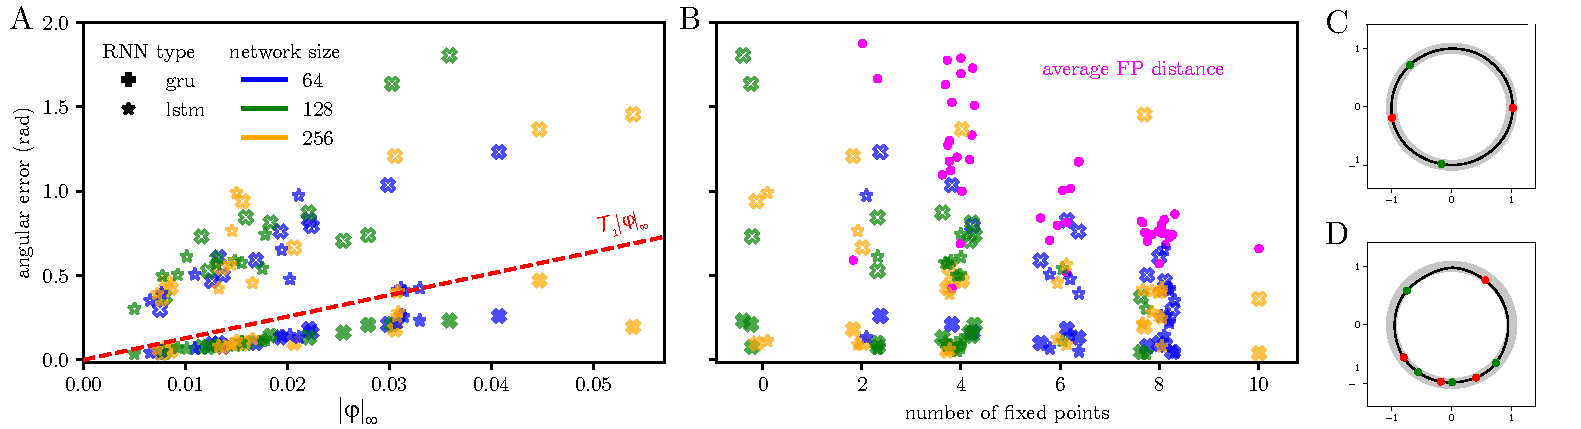
\includegraphics[width=\textwidth]{angular_losses_lstm_gru}
  \caption{The different measures for memory capacity reflect the generalization properties implied by the topology of the found solution.
    \textbf{(A)} The average accumulated angular error versus the uniform norm on the vector field shown for finite time (time of trial length on which networks were trained, \(T_1\)) indicated with filled markers and at asymptotic time (with hollow markers).
    \textbf{(B)}   The number of fixed points versus average accumulated angular error, with the average distance between neighbouring fixed points indicated in magenta.
}\label{fig:angular_losses_lstm_gru}
\end{figure}
%A==A
%B==C in main text

\end{document}